% Preamble
\documentclass[fleqn,10pt]{SelfArx}

\usepackage[english]{babel}
\usepackage{xcolor}
\setlength{\columnsep}{0.55cm}
\setlength{\fboxrule}{0.75pt} 
\definecolor{color1}{RGB}{0,0,90}
\definecolor{color2}{RGB}{0,20,20}
\usepackage{hyperref}
\hypersetup{
	hidelinks,
	colorlinks,
	breaklinks=true,
	urlcolor=color2,
	citecolor=color1,
	linkcolor=color1,
	bookmarksopen=false,
	pdftitle={Title},
	pdfauthor={Author},
}
\usepackage{nameref}

\usepackage{lipsum}
\usepackage{graphicx}
\usepackage{booktabs}
\usepackage{cite}
\usepackage{dblfloatfix}  % fix bottom placement
\usepackage{amsmath,amssymb}
\usepackage{enumitem}
\usepackage{booktabs,multirow}
\usepackage[font=small,labelfont=bf,skip=6pt]{caption}
\usepackage{float}
\graphicspath{{../results/data/plots/}}

\JournalInfo{JHU/EP EN.625.687.3VL.SP25 Applied Topology}
\Archive{Final Report}
\PaperTitle{Tomato TDA}
\Abstract{
    Given a finite metric space \((X,d)\) induced by text encodings (BoW, TF–IDF, BERT) and metrics (Cosine, Minkowski, Sinkhorn–Wasserstein, Geodesic), we build Vietoris–Rips filtrations \(\mathrm{VR}(X;\varepsilon)\) and compute persistent homology in degrees \(n=0,1,2\). In total, we assess 54 embedding/metric combinations and perform topological data analysis (TDA) on 270 metric spaces. 
}
\Authors{Morgan Bounds\textsuperscript{1}, Lianghao Chen\textsuperscript{1}, Clinten Graham\textsuperscript{1}} % Authors
\affiliation{\textsuperscript{1}\textit{JHU EP}} % Author affiliation

\Keywords{}
\newcommand{\keywordname}{Keywords}


\begin{document}

\maketitle
\tableofcontents % Output the contents section

\section{Methodology}

\subsection{Repository}
We used NumPy arrays for data and boundary matrices \cite{harris2020array}, computed barcodes via Ripser \cite{bauer2021ripser}, manipulated and visualized diagrams with Persim \cite{persim2024persim}, and evaluated Wasserstein distances using the POT optimal‐transport toolbox \cite{flamary2021pot}.
\subsection{Data Set}

\subsubsection{Stratification}

\subsection{Real Embeddings}
We mostly consider a single reviews to be single points embedded in $\mathbb{R}^d$, except for when we use metrics based on \nameref{ws}.
\subsection{Metric Spaces}
To apply TDA, we require a notion of distance between points (reviews) in our feature space, since persistent homology typically operates on a metric space \cite{edelsbrunner2009computational}.
\subsubsection{Cosine Distance}
Given two vectors $x, y \in \mathbb{R}^d$, we obtain their angle using the dot product $\langle x, y\rangle  = |x||y|\cos(\theta).$
This is converted to a distance via 
$$d_{\cos}(x,y) = \sqrt{2\left(1 - \cos(\theta)\right)} \in [0,2].$$
Cosine distance focuses on the difference in direction of the vectors, effectively comparing the relative term weights. For TF–IDF or BoW, this is useful because it reduces the influence of document length or overall word frequency. 
\subsubsection{Minkowski Distances}
A broad family of distances defined as 
$$d_p(x,y) = \Big(\sum_{i=1}^d |x_i - y_i|^p \Big)^{1/p}$$
for $p\ge1$ satisfy the metric axioms \cite{viro2008elementary}. We consider two important cases:
\begin{itemize}
	\item \textbf{Manhattan distance} ($\ell_1$ norm, with $p=1$)
	$$d_{1}(x,y) = \sum_{i}|x_i - y_i|$$
	If $x,y$ are BoW vectors, $d_1$ counts the total difference in word counts between two reviews. This can be more robust than Euclidean ($p=2$) to high-dimensional sparse differences, since it doesn’t overly emphasize large single-component differences (instead, it treats each dimension linearly).
	\item \textbf{Chebyshev distance} ($\ell_{\infty}$ norm, the limit as $p \to \infty$)
	$$d_{\infty}(x,y) = \max_i |x_i - y_i|$$
	In text, $d_{\infty}$ might be interpreted as looking at the word with the most disproportionate frequency between two reviews. For example, if one review heavily uses the word “excellent” and another does not use it at all, Chebyshev distance would equal the normalized frequency difference for "excellent".
\end{itemize}

\section{Full Structure}
\subsubsection{Characterization}
On each normalized diagram we compute total persistance and persistant entropy,
\begin{align*}
	\operatorname{TP}_k(X)&=\sum_{\left(b_i, d_i\right) \in \operatorname{Dgm}_k(X)}\left(d_i-b_i\right)=\int_0^{\alpha_{\max }} \beta_k(\alpha) d \alpha\\
	\operatorname{E}_k(X)&=\sum_{\left(b_i, d_i\right) \in \operatorname{Dgm}_k(X)}-p_i\log(p_i), \quad p_i=\frac{d_i-b_i}{\sum_j\left(d_j-b_j\right)}
\end{align*}
capturing overall lifetime and dispersion of features \cite{adams2017persistence}.

\begin{figure*}[t]
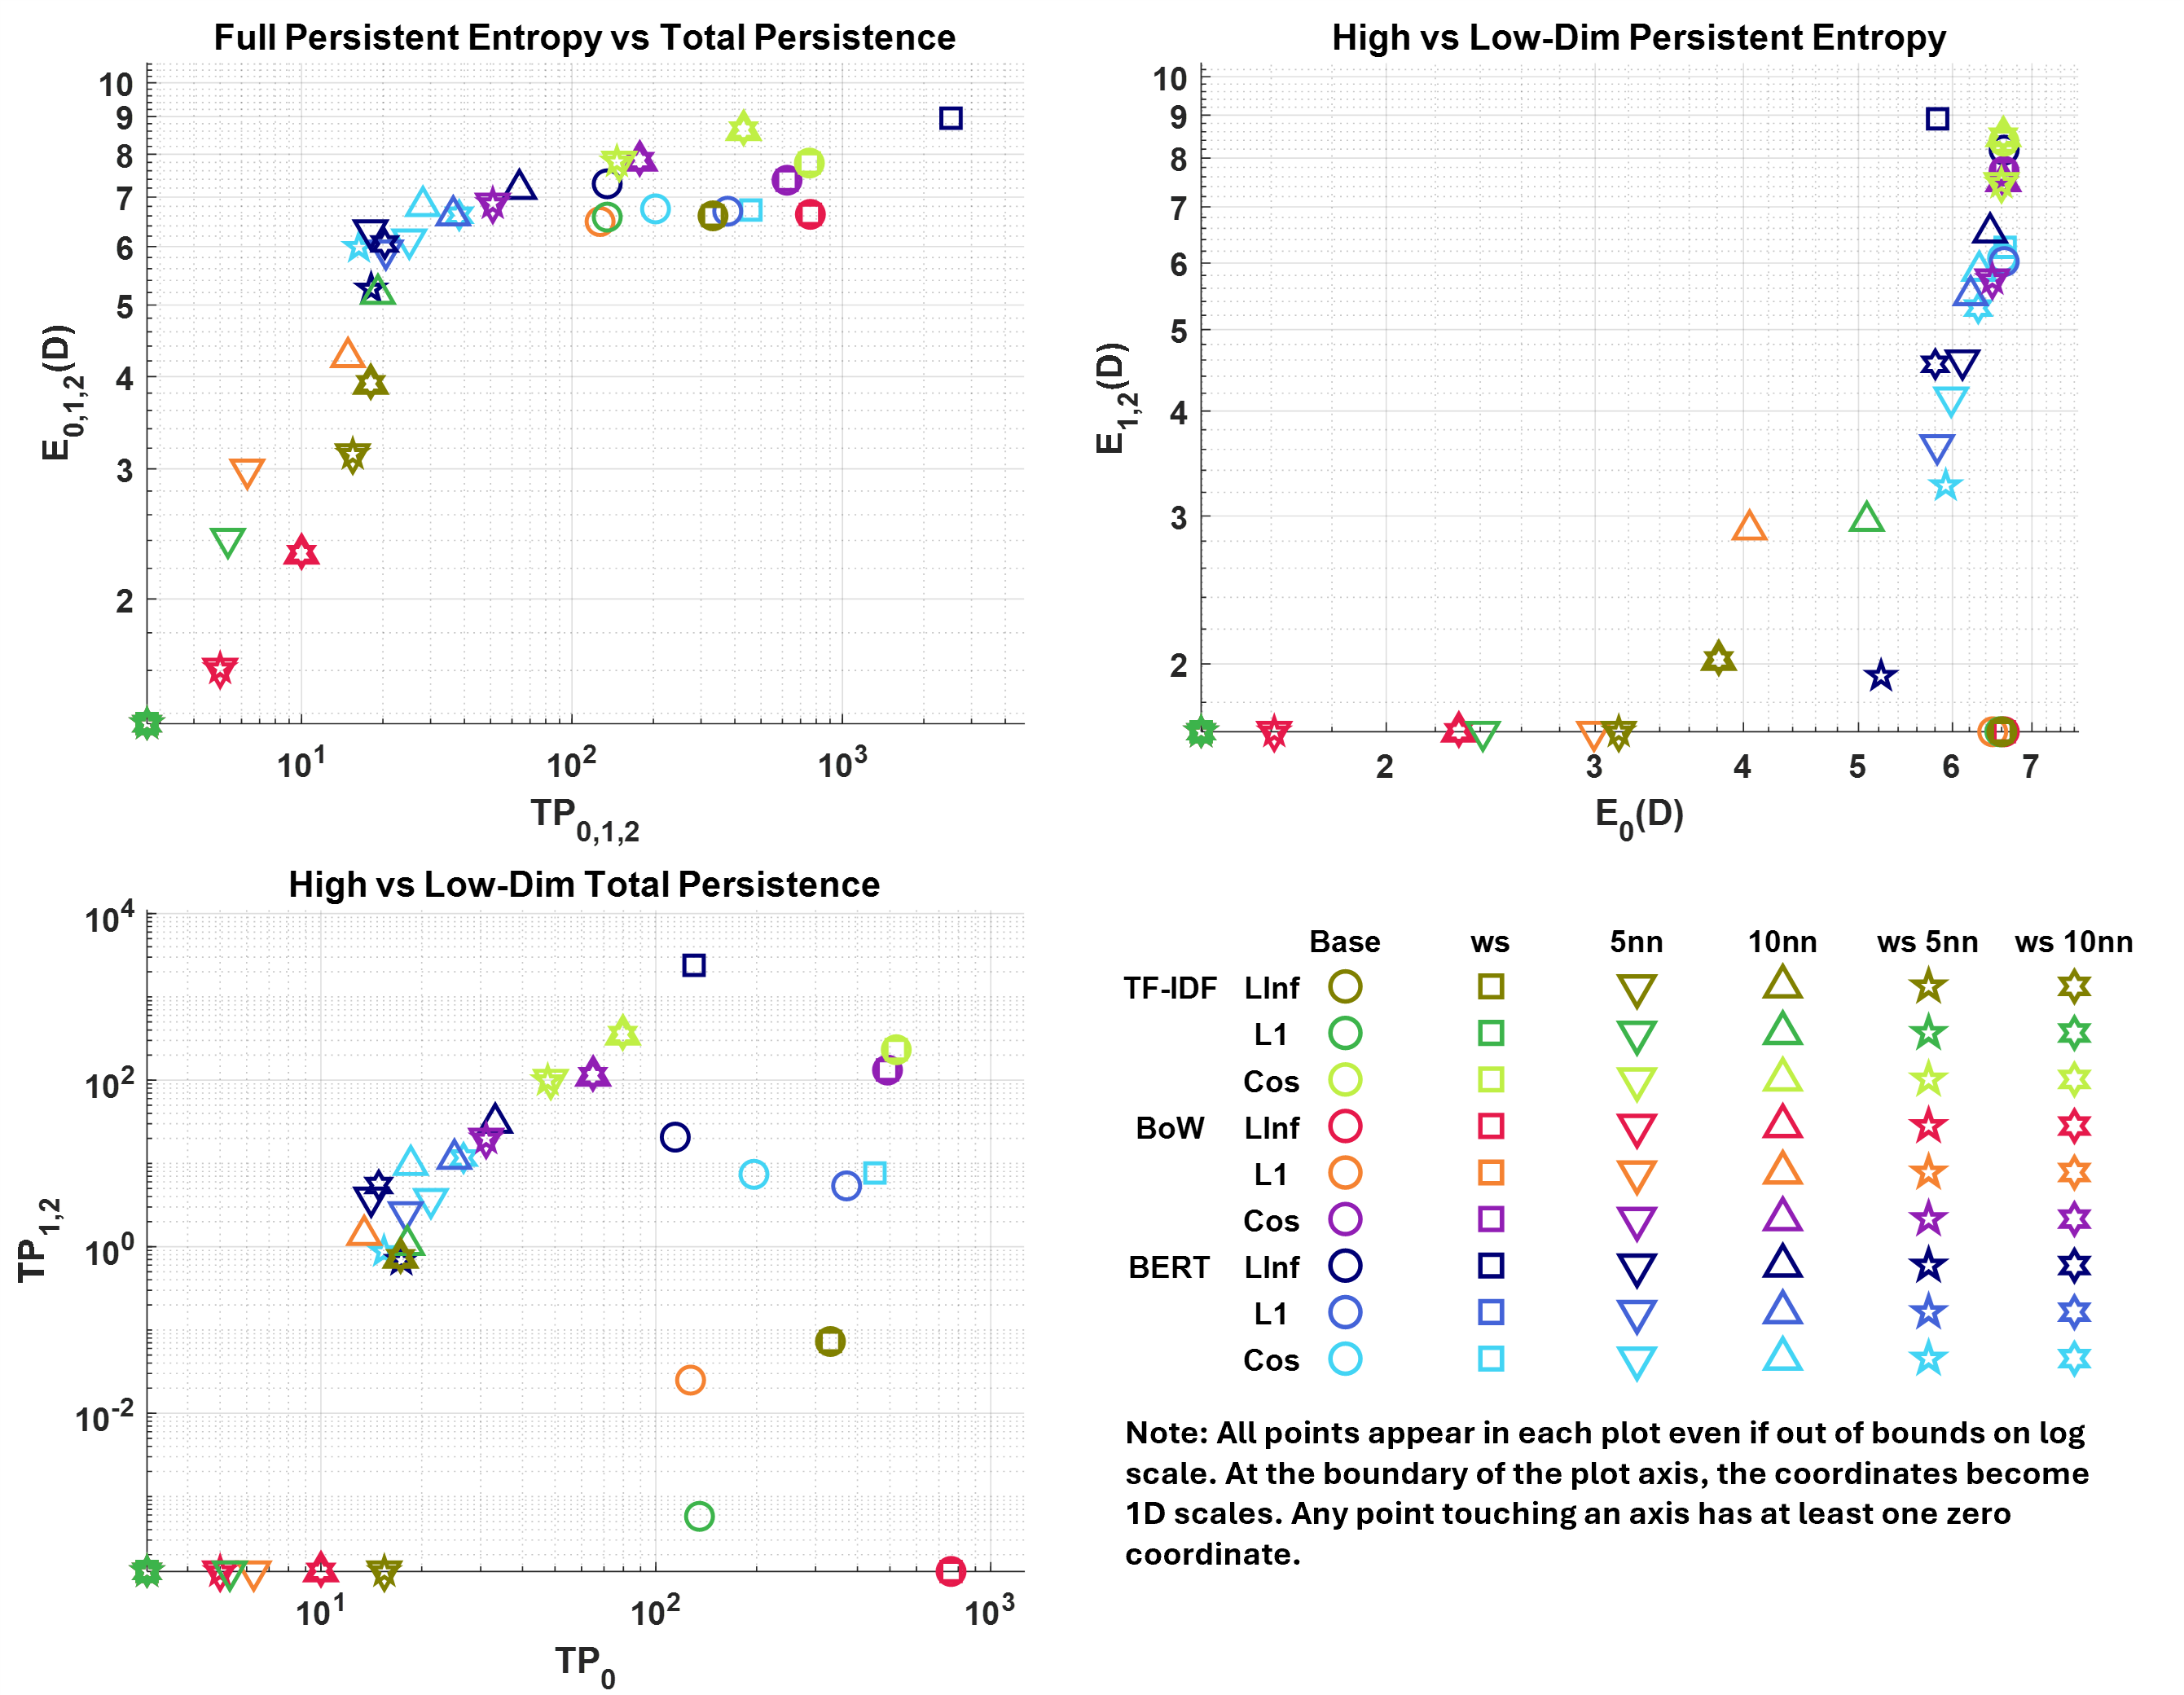
\includegraphics[width=\textwidth]{comparative/general/FullStructureV2.png}
\caption{bla bla}
\label{fig:FullStructure}
\end{figure*}
% discuss extrema (deep dive persistance)

% different embedding lead to different structure

\section{Discriminating Structure}
% define axes of discrimination
\begin{figure*}[t]
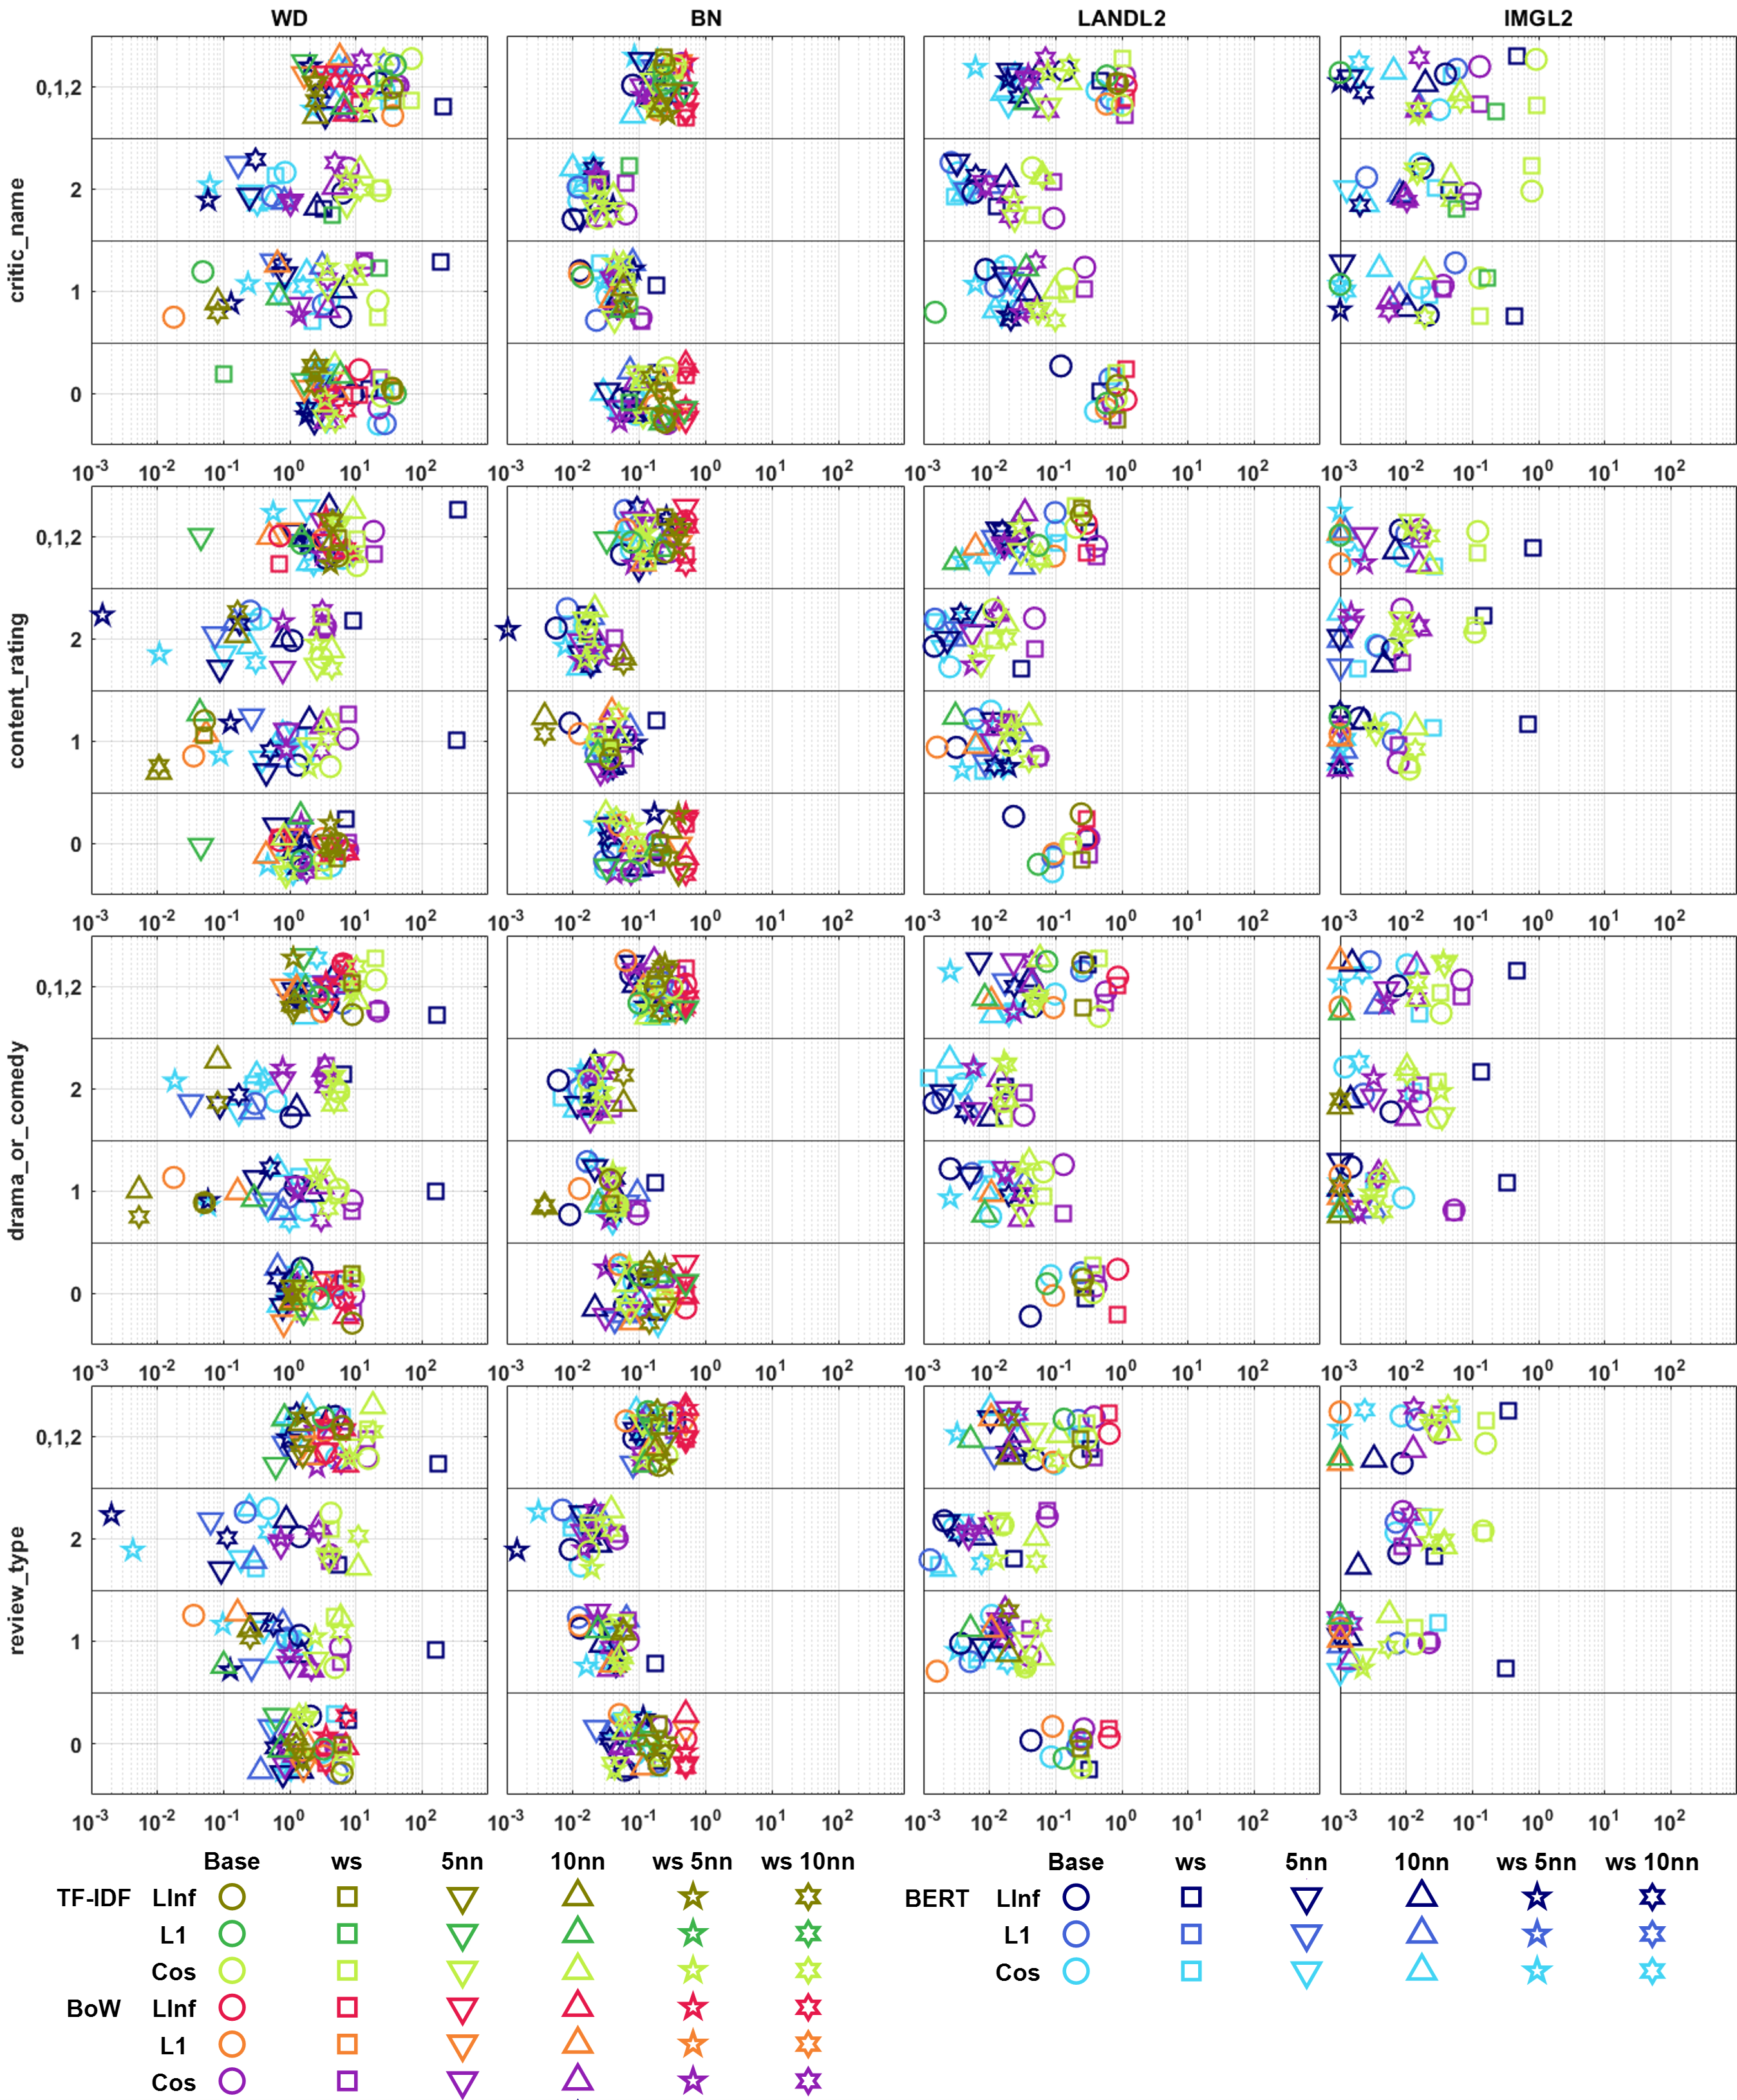
\includegraphics[width=\textwidth]{comparative/general/DiscrimStructureV2.png}
\caption{bla bla}
\label{fig:DiscrimStructure}
\end{figure*}
% discuss extrema (deep dive persistance)

\begin{table*}[t]
	\centering
	\begin{tabular}{ccccr}
	\toprule
	\textbf{Category} & \textbf{Dim} & \textbf{Encoding} & \textbf{Top Metric} & \textbf{Discrim.} \\
	\midrule
	\multirow{4}{*}{Drama or comedy}
	 & 0   & BoW   & Cosine                          & 9.3   \\
	 & 1   & BERT  & Minkowski $p=\infty$             & 158.5 \\
	 & 2   & BERT  & Minkowski $p=\infty$             & 6.6   \\
	 & 012 & BERT  & Minkowski $p=\infty$             & \textbf{171.9} \\
	\midrule
	\multirow{4}{*}{Review type}
	 & 0   & BERT  & Minkowski $p=\infty$             & 7.7   \\
	 & 1   & BERT  & Minkowski $p=\infty$             & 160.7 \\
	 & 2   & TF-IDF & Cosine + Wasserstein + 10NN Isomap & 10.9  \\
	 & 012 & BERT  & Minkowski $p=\infty$             & \textbf{173.8} \\
 	\midrule
 	\multirow{4}{*}{Critic name}
	 & 0   & TF-IDF & Minkowski $p=1$                  & 39.5  \\
	 & 1   & BERT  & Minkowski $p=\infty$             & 191.7 \\
	 & 2   & TF-IDF & Cosine                           & 23.3  \\
	 & 012 & BERT  & Minkowski $p=\infty$             & \textbf{211.0} \\
	 	\midrule
	 	\multirow{4}{*}{Content rating}
	 & 0   & BoW   & Cosine                          & 7.5   \\
	 & 1   & BERT  & Minkowski $p=\infty$             & 331.6 \\
	 & 2   & BERT  & Minkowski $p=\infty$             & 8.9   \\
	 & 012 & BERT  & Minkowski $p=\infty$             & \textbf{347.6} \\
	\bottomrule
	\end{tabular}
	\caption{Best metrics and max discriminability scores by category and dimension.}
	\label{tab:best-metrics}
\end{table*}

\subsection{Observation 1: Schwartz}
% define axes of discrimination
% plot
% discuss extrema (deep dive persistance)

\begin{figure}[h]
\centering
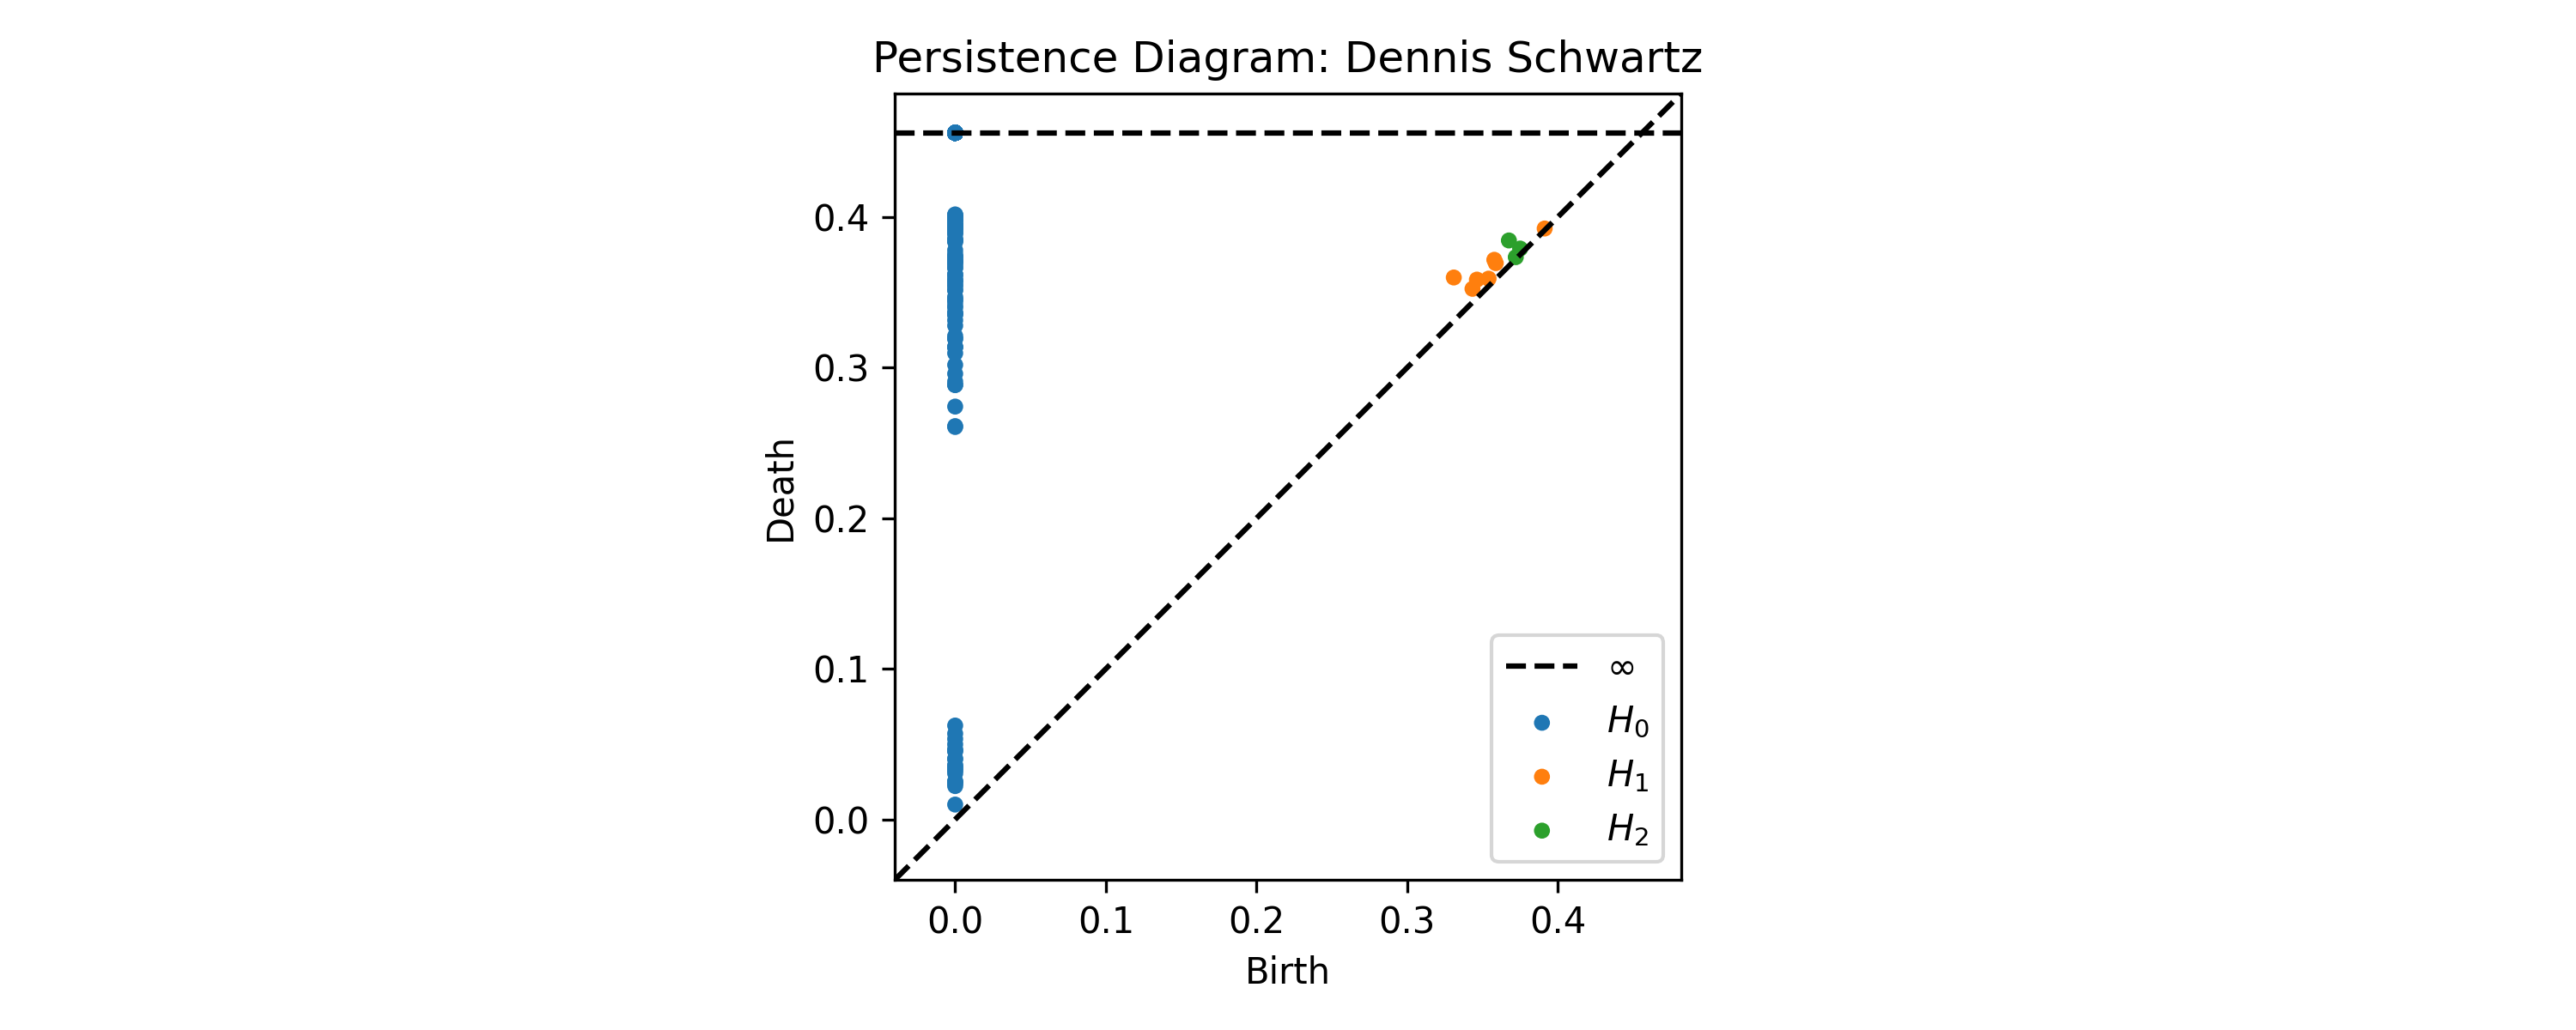
\includegraphics[trim={6cm 0 6cm 0},clip,width=\columnwidth]{critic_name/Dennis Schwartz_diagram.png}
\caption{Persistence diagram for Dennis Schwartz's reviews showing birth-death pairs of topological features. Note the presence of 7 dimension-1 features (loops) and 3 dimension-2 features (voids), indicating non-trivial topological structure in the embedding space.}
\label{fig:schwartz_diagram}
\end{figure}

\begin{figure}[h]
\centering

\includegraphics[width=\columnwidth]{critic_name/betti_curves_H1.png}
\caption{Betti curves showing the persistence of 1-dimensional homology features (loops) across different filtration values for both critics. Dennis Schwartz's reviews demonstrate more persistent loops, suggesting a more complex topological structure.}
\label{fig:betti_curves}
\end{figure}

The topological analysis of movie reviews written by Dennis Schwartz reveals intriguing structures in the BERT embedding space. As shown in Figure \ref{fig:schwartz_diagram}, Schwartz's reviews demonstrate a notable presence of higher-dimensional topological features, with 7 dimension-1 features (loops) and 3 dimension-2 features (voids). The maximum persistence value for dimension-1 features is 0.029, while for dimension-2 features it is 0.017, indicating reasonably stable topological structures.

This non-trivial topology suggests that Schwartz's critical language forms distinct clusters with interconnections, creating loop structures that likely represent recurring thematic elements or linguistic patterns in his reviews. The presence of these loops implies that Schwartz's critical style may orbit around certain conceptual centers before returning to common reference points or perspectives—a pattern consistent with a critic developing signature analytical frameworks.

Comparing the Betti curves in Figure \ref{fig:betti_curves}, we observe that Schwartz's reviews maintain higher persistence in dimension-1 features compared to Roger Ebert's reviews. This suggests that Schwartz may employ a more structured approach to criticism, with greater consistency in how he frames and develops his arguments across different films.

The dimension-2 features (voids) are particularly interesting, as they indicate three-dimensional "bubbles" in the semantic space. These voids might represent conceptual boundaries in Schwartz's criticism—areas where he deliberately avoids certain types of analysis or language. Alternatively, they could reflect a tendency to approach films from multiple contrasting perspectives, creating a more spherical structure in semantic space as his analysis encircles the subject from different angles.

From a stylistic perspective, these topological features may correlate with Schwartz's writing style, which tends to balance academic analysis with accessible criticism. The presence of both loops and voids suggests a critic who returns to foundational principles while maintaining conceptual distinctions between different types of films or critical approaches.

\begin{figure}[h]
\centering

\includegraphics[width=\columnwidth]{comparative/critic_name/bottleneck_heatmap.png}
\caption{Bottleneck distance heatmap between different critics. The distance of 0.197 between Dennis Schwartz and Roger Ebert indicates meaningful topological distinctions in their critical approaches.}
\label{fig:bottleneck_distance}
\end{figure}

The bottleneck distance of 0.197 between Schwartz and Ebert (Figure \ref{fig:bottleneck_distance}) quantifies the difference in their topological signatures. This substantial distance suggests fundamentally different cognitive frameworks between the two critics, despite reviewing the same films. This divergence likely reflects different priorities in their evaluations and distinct rhetorical strategies in their writing.

Notably, the Betti curves (Figure \ref{fig:betti_curves}) exhibit a distinctive spike for Dennis Schwartz's reviews at a filtration value of approximately 0.05. This sharp increase indicates a threshold at which many loops simultaneously form in the embedding space, suggesting a critical distance at which Schwartz's language patterns suddenly connect to create circular semantic structures. This abrupt topological transition might correspond to a characteristic scale at which Schwartz's critical vocabulary forms conceptual relationships—perhaps indicating a distinctive granularity at which his analytical framework operates most coherently. The spike's height and narrowness suggest these structures form rapidly and in large numbers at this specific scale, potentially revealing a fundamental frequency in his linguistic patterns or conceptual organization that distinguishes his critical voice.

\clearpage
\subsection{Preferred Metric}
% Differences heatmap

\section{Conclusions}

\phantomsection
\bibliographystyle{unsrt}
\bibliography{tda.bib}
\end{document}